% {\Large \textbf{Mechanical:}}
\qns{Coordinate Change Practice}
\qcontributor{Yi Zhao}

Many engineering problems are modeled as linear systems.
These linear systems usually are hard to solve in its original basis.
However, the same systems are much easier to solve if we change to a new basis.
In this problem, we will try to review the \emph{change of basis} for vectors.
We can represent a \emph{change of basis} by a square and invertible matrix.
\par

Let's first start with an example.
Consider the vector $\vec{u} = \begin{bmatrix} u_1 \\ u_2 \end{bmatrix}$.
When we write a vector in this form, implicitly we are representing it in the \emph{standard basis} for $\R^{2}$, $\vec{e_1} = \begin{bmatrix} 1 \\ 0 \end{bmatrix}$ and $\vec{e_2} = \begin{bmatrix} 0 \\ 1 \end{bmatrix}$.
This means that we can write $\vec{u} = u_1\vec{e_1} + u_2\vec{e_2}$.
\par

What if we want to represent $\vec{u}$ as a linear combination of another set of basis vectors, say $\vec{a_1} = \begin{bmatrix} 1 \\ 1 \end{bmatrix}$ and $\vec{a_2} = \begin{bmatrix} 0 \\ -1 \end{bmatrix}$?
This means that we need to find scalars $u_{a_1}$ and $u_{a_2}$ such that $\vec{u} = u_{a_1}\vec{a_1} + u_{a_2}\vec{a_2}$.
We can write this equation in matrix form:
\[
  \begin{bmatrix}
    | & | \\
    \vec{a_1} & \vec{a_2} \\
    | & |
  \end{bmatrix}
  \begin{bmatrix} u_{a_1} \\ u_{a_2} \end{bmatrix} = \begin{bmatrix} u_{1} \\ u_{2} \end{bmatrix}
.\]
Thus we can find $u_{a_1}$ and $u_{a_2}$ by solving a system of linear equations.
\par


\begin{enumerate}

\qitem Let $\vec{v} = [2,-1]^{T}$. What equation gives the coordinates of $\vec{v}$ in the below basis?

\begin{gather*}
\vec{x} =
\begin{bmatrix}
4 \\
-2
\end{bmatrix},
\vec{y} = \begin{bmatrix}
-3 \\
-3
\end{bmatrix}
\end{gather*}

\meta{


  Now that we know how to change the basis of vectors, let's shift our attention to linear transformations.
  Suppose we have a linear transformation $T$ represented by a $n \times n$ matrix that transforms $\vec{u} \in \R^{n}$ to $\vec{v} \in \R^{n}$:
  \[
    \vec{v} = T\vec{u}
  .\]
  Suppose we have a basis vectors $\vec{a_1}, \cdots, \vec{a_n} \in \R^{n}$, and the vectors $\vec{u}, \vec{v}$ above are represented in this basis:
  \[
    \begin{aligned}
      \vec{u_a} &= u_{a_1}\vec{a_1} + \cdots + u_{a_n}\vec{a_n} \\
      \vec{v_a} &= v_{a_1}\vec{a_1} + \cdots + v_{a_n}\vec{a_n}.
    \end{aligned}
  \]
  Thus we have
  \[
    \begin{aligned}
      T\vec{u}          &= \vec{v} \\
      TA\vec{u_a}       &= A\vec{v_a} \\
      A^{-1}TA\vec{u_a} &= \vec{v_a}.
    \end{aligned}
  \]
  By pattern matching, we see that if we set $T_a = A^{-1}TA$, we get the relationship $T_a\vec{u_a} = \vec{v_a}$ in the new basis.
  The correspondences stated above are all represented in the following diagram:
  % \begin{figure}[H]
  %   \centering
  %   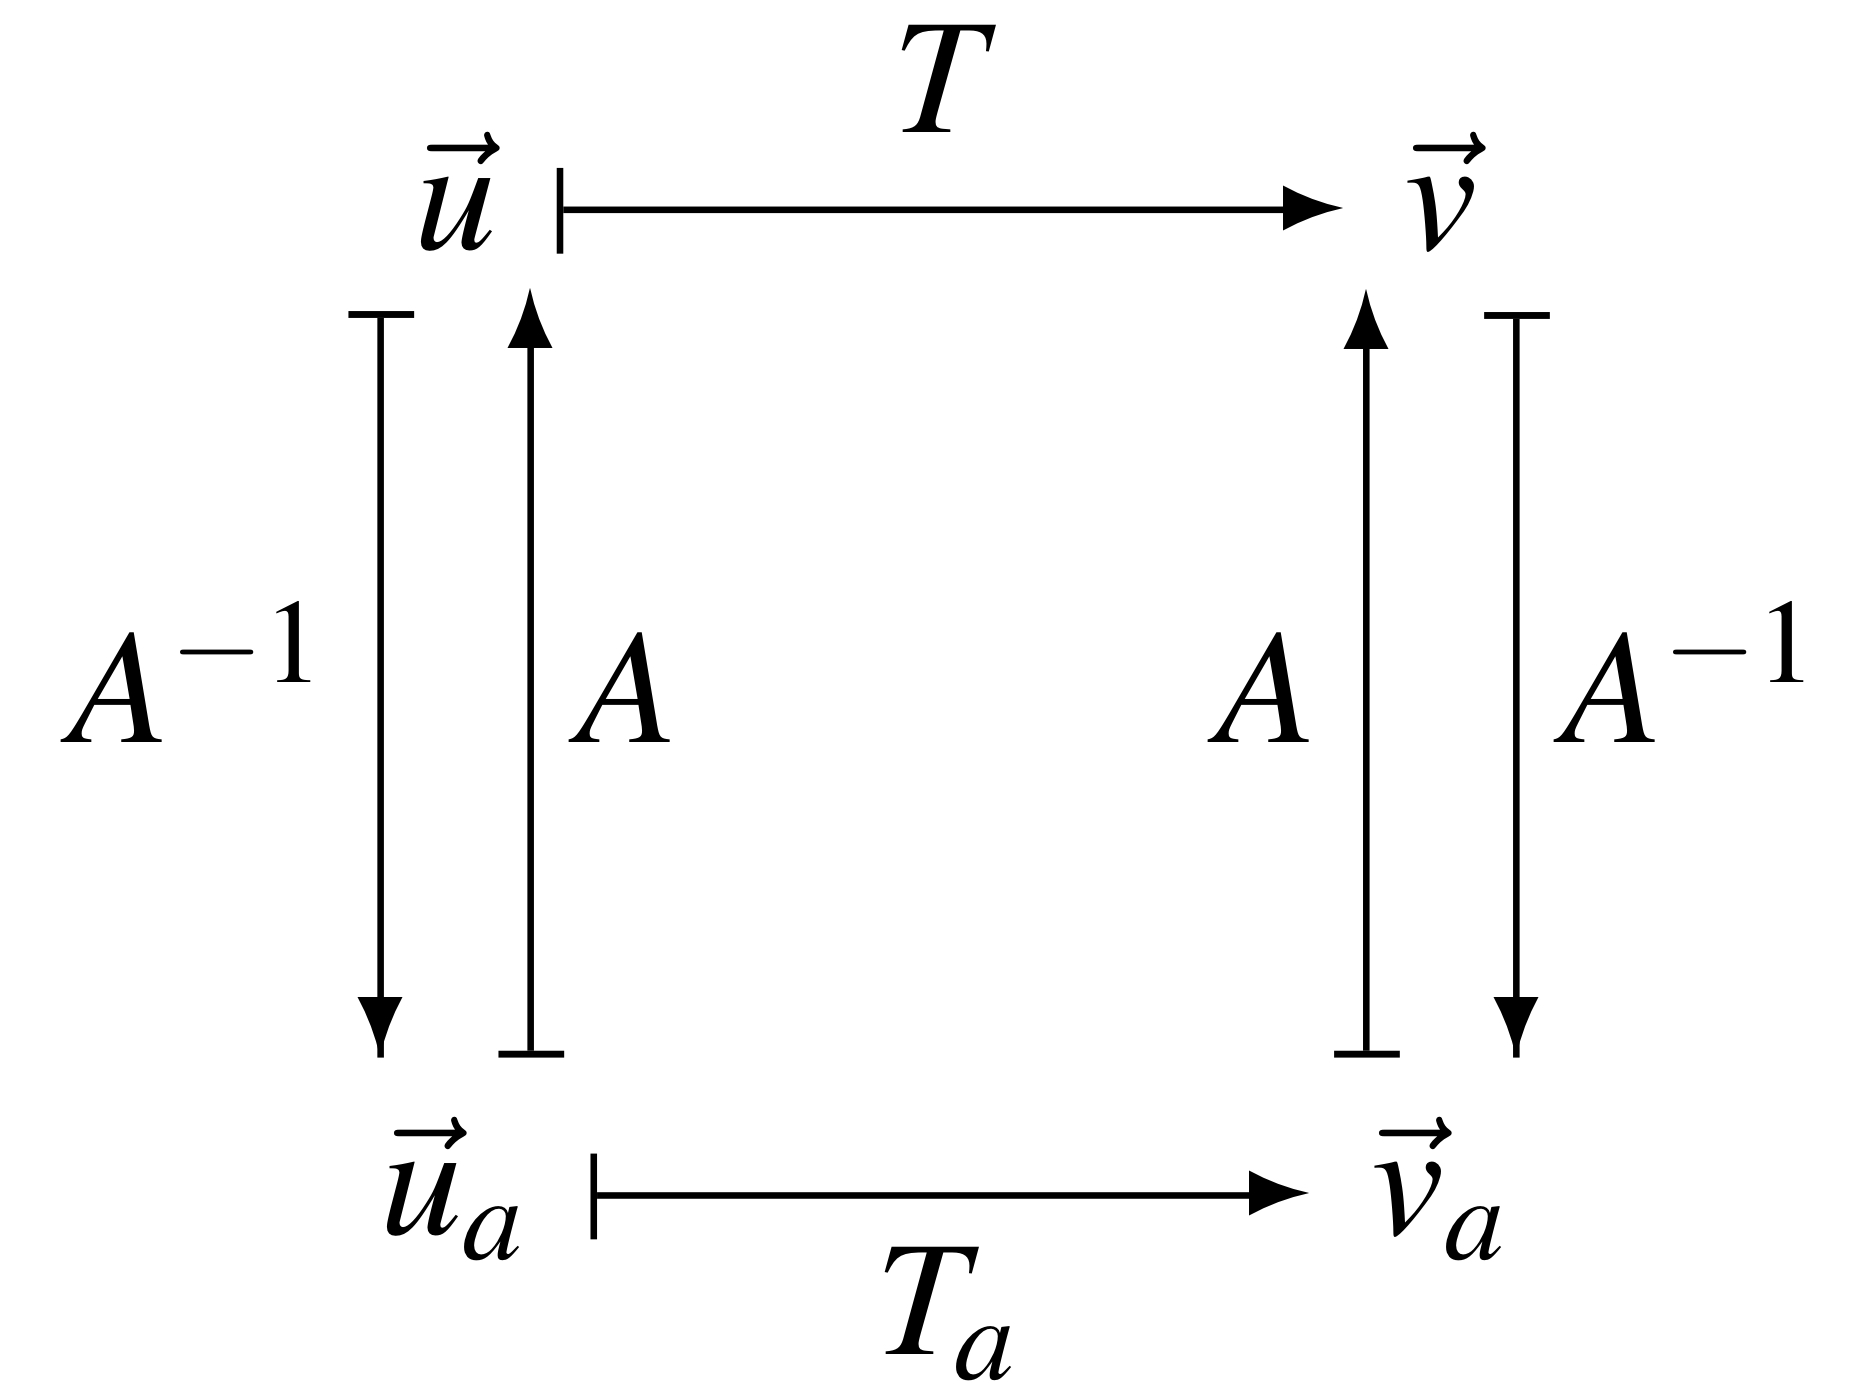
\includegraphics[scale=0.1]{\bank/statespace/figures/change_of_basis.jpg}
  % \end{figure}

  \begin{figure}[H]
    \centering
    \begin{tikzpicture}[node distance = 2cm, thick]%
      \node (1) {$\vec{u}$};
      \node (2) [right=of 1] {$\vec{v}$};
      \node (3) [below=of 2] {$\vec{v_a}$};
      \node (4) [below=of 1] {$\vec{u_a}$};
      \draw[->] (1) -- node [midway,above] {$T$} (2);
      \draw[->] (1.240) -- node [midway,left]{$A^{-1}$} (4.120);
      \draw[->] (4.60) -- node [midway,right]{$A$} (1.300);
      \draw[->] (2.300) -- node [midway,right]{$A^{-1}$} (3.60);
      \draw[->] (3.120) -- node [midway,left]{$A$} (2.240);
      \draw[->] (4) -- node [midway,below] {$T_a$} (3);
    \end{tikzpicture}%
  \end{figure}

}


\sol{

  In general, suppose we are given a vector $\vec{u} \in \R^{n}$ in the standard basis and want to change to a different basis with linearly independent basis vectors $\vec{a_1}, \cdots, \vec{a_n}$.
  If we denote the vector in the new basis as $\vec{u_a} = \begin{bmatrix} u_{a_1} \\ \vdots \\ u_{a_n} \end{bmatrix}$, we solve the following equation $A\vec{u_a} = \vec{u}$, where A is the matrix $\begin{bmatrix} \vec{a_1} & \cdots & \vec{a_n} \end{bmatrix}$.
  Therefore the change of basis is given by:
  \[
    \vec{u_a} = A^{-1}\vec{u}
  .\]

    $$
        \vec{c} =
        \begin{bmatrix}
        4 & -3 \\
        -2 & -3
        \end{bmatrix}^{-1}
        \begin{bmatrix}
        2 \\
        -1
        \end{bmatrix}
        $$
}


\qitem Let $\vec{v} = [3,3]^{T}$. We are told that $\vec{v}$ is represented in the basis:

\begin{gather*}
\vec{x} =
\begin{bmatrix}
1 \\
1
\end{bmatrix},
\vec{y} = \begin{bmatrix}
1 \\
-1
\end{bmatrix}
\end{gather*}
What equation gives the coordinates of $\vec{v}$ in the standard basis?

\sol {
  If we already have a vector $\vec{u_a}$ in the basis $\vec{a_1}, \cdots, \vec{a_n}$, how do we change it back to a vector $\vec{u}$ in the standard basis?
  We can reverse the change of basis transformation, thus $\vec{u} = A\vec{u_a}$.
  \par

    $$
        \vec{c} =
        \begin{bmatrix}
        1 & 1 \\
        1 & -1
        \end{bmatrix}
        \begin{bmatrix}
        3 \\
        3
        \end{bmatrix}
        $$
}

\bigskip

\begin{adjustwidth}{-20pt}{0pt}

For many problems (eg. solving a system of differential equations), it is useful to change to the eigenbasis. \\
For instance, if we have vectors $\vec{x_1}$ and $\vec{x_2}$ that are related by $\vec{x_2} = A \vec{x_1}$, we would want to change to a basis represented by the eigenvectors of $A$.
If $$A \vec{v_1} = \lambda_1 \vec{v_1}, A \vec{v_2} = \lambda_2 \vec{v_2}, \dots, A\vec{v_n} = \lambda_n \vec{v_n} $$
our change of basis matrix would be
$$ V =
\begin{bmatrix}
\vec{v_1} & \vec{v_2} & \dots & \vec{v_n}
\end{bmatrix}
$$

This change of basis is called diagonalization because $\vec{x_1}'$ and $\vec{x_2}'$ (representations of $\vec{x_1}$ and $\vec{x_2}$ in the V-basis) are related by
$$ \vec{x_2}' =
\begin{bmatrix}
\lambda_1 & 0 & \dots & 0 \\
0 & \lambda_2 & \dots & 0 \\
\vdots & \vdots & \ddots & \vdots \\
0 & 0 & \dots & \lambda_n
\end{bmatrix} \vec{x_1}'
$$ \\
A matrix in $\mathbb{R}^{n}$ is diagonalizable if it has $n$ linearly independent eigenvectors (i.e. the $V$ matrix is invertible).

\end{adjustwidth}

\bigskip

\qitem Let $\vec{x_2}$ be the result when a linear transformation is applied on $\vec{x_1}$.
$$\vec{x_2} = A \vec{x_1} =
\begin{bmatrix}
3 & -1 \\
-2 & 4
\end{bmatrix}
\vec{x_1}
$$

where $x_1$ and $x_2$ are in the standard basis. \\
Now, let us change to the eigenbasis of $A$, represented by $\vec{v_1}$ and $\vec{v_2}$
$$
\vec{v_1} =
\begin{bmatrix}
1 \\
-2
\end{bmatrix},
\vec{v_2} =
\begin{bmatrix}
1 \\
1
\end{bmatrix}
$$

$$ V =
\begin{bmatrix}
\vec{v_1} & \vec{v_2}
\end{bmatrix}
$$

Suppose $\vec{z_1}$ and $\vec{z_2}$ are the representations of $\vec{x_1}$ and $\vec{x_2}$ in the eigenbasis.
So, $\vec{z_1} = V^{-1}\vec{x_1}$ and $\vec{z_2} = V^{-1}x_2$.
We see that $\vec{z_1}$ and $\vec{z_2}$ are related by $\vec{z_2} = A'\vec{z_1}$.
What is the matrix $A'$? \\
\textit{
Write your answer in terms of matrix multiplications.
Given $\lambda_1 = 5$ and $\lambda_2 = 2$, what are the elements of $A'$?
} \\
\sol{
    Start by writing $\vec{x_1}$ in terms of $\vec{z_1}$:
    $$ \vec{x_1} = V \vec{z_1} $$
    Then, apply the transformation $A$ to $\vec{x_1}$, substituting $V \vec{z_1}$ for $\vec{x_1}$:
    $$ \vec{x_2} = A V \vec{x_1} $$
    Finally, left-multiply both sides by $V^{-1}$ to change $\vec{x_2}$ to the eigenbasis:
    $$ \vec{z_2} = V^{-1} \vec{x_2} = V^{-1} A V \vec{z_1} $$

    $$A' = V^{-1} A V =
    \begin{bmatrix}
    1 & 1 \\
    -2 & 1
    \end{bmatrix}^{-1}
    \begin{bmatrix}
    3 & -1 \\
    -2 & 4
    \end{bmatrix}
    \begin{bmatrix}
    1 & 1 \\
    -2 & 1
    \end{bmatrix}
    $$

    $A'$ represents the transformation $A$ in the eigenbasis of $A$, so we know that $A'$ is the diagonal matrix:
    $$ A' =
    \begin{bmatrix}
    \lambda_1 & 0 \\
    0 & \lambda_2
    \end{bmatrix} =
    \begin{bmatrix}
    5 & 0 \\
    0 & 2
    \end{bmatrix} $$
}

\qitem \textbf{True or False}: If a matrix is invertible, it can be diagonalized. \\
\sol{ False, there are some matrices that are invertible but not diagonalizable.

}

\qitem \textbf{True or False} There is a unique eigenvalue decomposition for any matrix. \\
\sol{False, you can always find a different basis that diagonalizes the matrix.}






\end{enumerate}
